% DO NOT COMPILE THIS FILE DIRECTLY!
% This is included by the other .tex files.

\begin{frame}[t,plain]
\titlepage
\end{frame}

\begin{frame}
	\frametitle{Authentication in Cerebrate}
	\begin{itemize}
                \item The goal is to give a quick explanation of how erebrate handles
                \begin{itemize}
                    \item Authentication
                    \item Access control
                    \item API vs UI differences
                    \item API key handling
                \end{itemize}
	\end{itemize}
\end{frame}

\begin{frame}
	\frametitle{Supported authentication methods}
	\begin{itemize}
                \item Implemented
                \begin{itemize}
                    \item Username/password
                    \item API key
                \end{itemize}
                \item Planned for the future
                \begin{itemize}
                    \item Integration with external IAM
                \end{itemize}
	\end{itemize}
\end{frame}

\begin{frame}
  \frametitle{MISP and Cerebrate}
  \begin{itemize}
      \item Code reuse for several authentication and ACL tasks
      \item Reuse of a lot of the prior work for MISP
      \item Allows us to save effort and reuse the work of the massive MISP dev community
      \item Because of this it's important to also talk about what's there in MISP
  \end{itemize}
\end{frame}

\begin{frame}
  \frametitle{Design philosophy}
  \begin{itemize}
      \item All endpoints in Cerebrate / MISP should work similarly via the UI and API
      \item Authentication via the UI and the API are separate
      \item In default mode, Cerebrate/MISP handles authentication
      \item When plugins are enabled / external IAM systems are attached, they take over optionally
      \begin{itemize}
          \item Flexible intermediary system for cases when no specific integration exists
          \item MISP only so far
          \item Cerebrate soon
      \end{itemize}
  \end{itemize}
\end{frame}

\begin{frame}
  \frametitle{Architecture}
  \begin{center}
    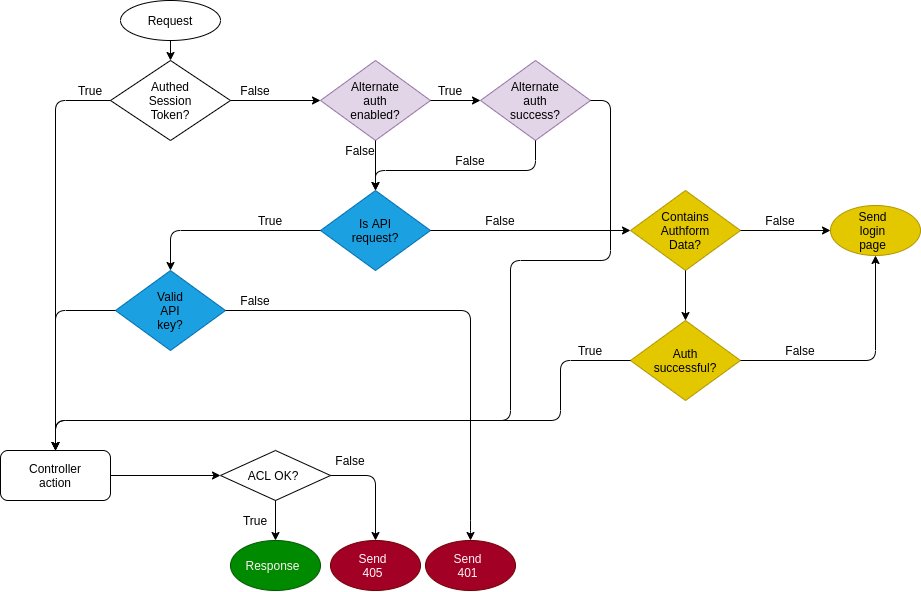
\includegraphics[scale=0.33]{Authentication.png}
  \end{center}
\end{frame}


\begin{frame}
  \frametitle{Potential plugins}
  \begin{itemize}
    \item IAM of choice for MC2 is an obvious choice
    \item Additional options foreseen
    \begin{itemize}
      \item Native LDAP?
      \item Native client side certificate
      \item Custom auth system from MISP
    \end{itemize}
  \end{itemize}
\end{frame}

\begin{frame}
  \frametitle{Custom authentication in MISP}
  \begin{itemize}
    \item Add a custom data point to user objects
    \item Tell MISP what header to expect
    \item Authenticate the user
    \item Potentially: Enroll the user in MISP/Cerebrate
  \end{itemize}
\end{frame}

\begin{frame}
  \frametitle{Enrollment}
  \begin{itemize}
    \item Most of these modules 
    \item Tell MISP what header to expect
    \item Authenticate the user
    \item Potentially: Enroll the user in MISP/Cerebrate
  \end{itemize}
\end{frame}

\begin{frame}
  \frametitle{Custom auth}
  \begin{center}
    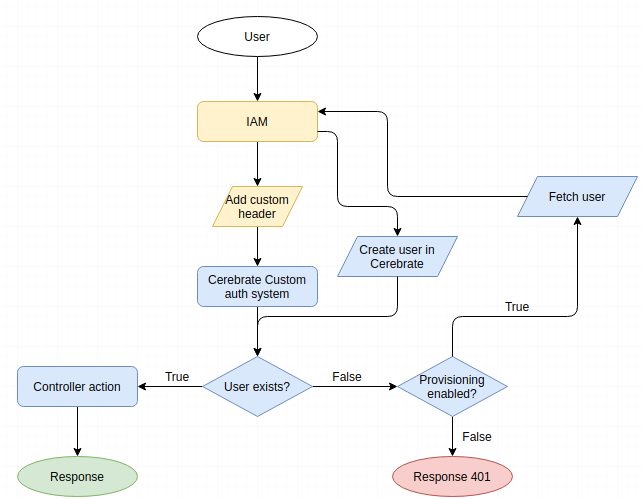
\includegraphics[scale=0.5]{customAuth.png}
  \end{center}
\end{frame}

\begin{frame}
  \frametitle{Custom auth configuration (MISP)}
  \begin{center}
    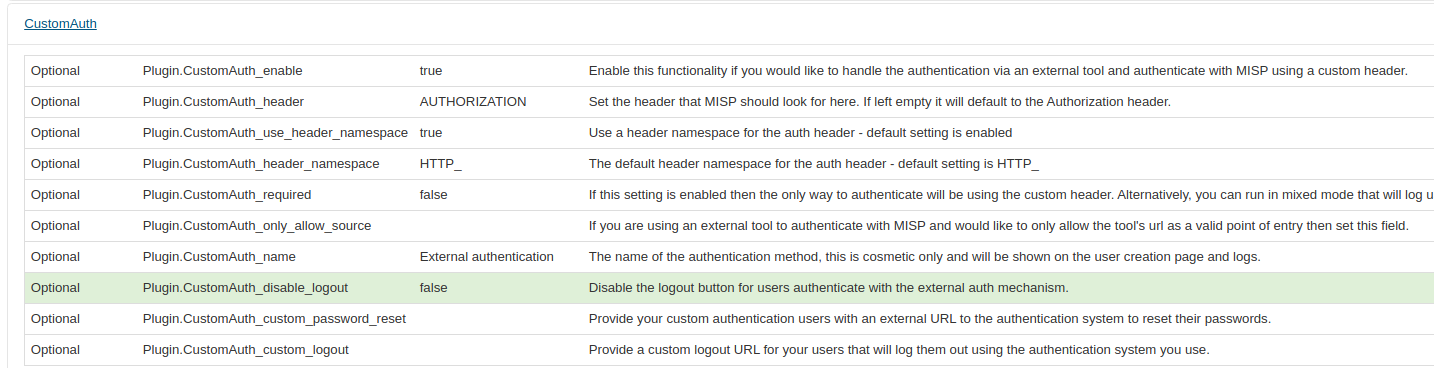
\includegraphics[scale=0.4]{customAuthSettings.png}
  \end{center}
\end{frame}

\begin{frame}
  \frametitle{API key management}
  \begin{itemize}
    \item Traditionally in MISP
    \begin{itemize}
      \item Single API key per user
      \item API key stored in the clear
    \end{itemize}
  \end{itemize}
\end{frame}

\begin{frame}
  \frametitle{Old style}
  \begin{center}
    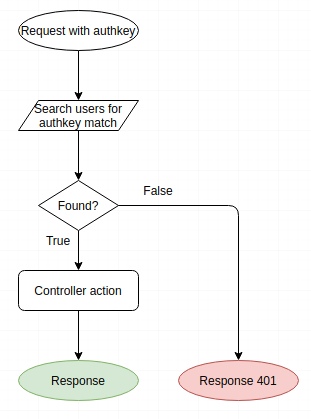
\includegraphics[scale=0.5]{simpleAuthkey.png}
  \end{center}
\end{frame}


\begin{frame}
  \frametitle{Reworked API key management for Cerebrate}
  \begin{itemize}
    \item Multiple API keys per user
    \item API keys can have comments to differentiate between usage (my other tool, my script)
    \item API keys are stored hashed (via bcrypt) with only the first and last 4 characters stored in the clear
    \item Keys can have expiration dates set
  \end{itemize}
\end{frame}

\begin{frame}
  \frametitle{New style}
  \begin{center}
    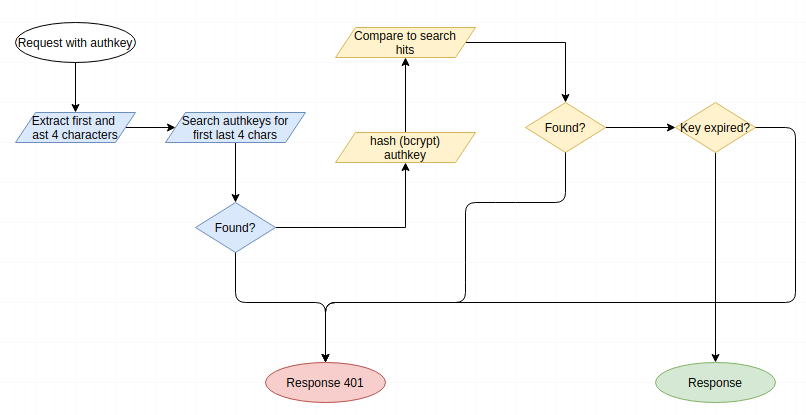
\includegraphics[scale=0.5]{advancedAuthkey.png}
  \end{center}
\end{frame}

\begin{frame}
  \frametitle{New style implementation}
    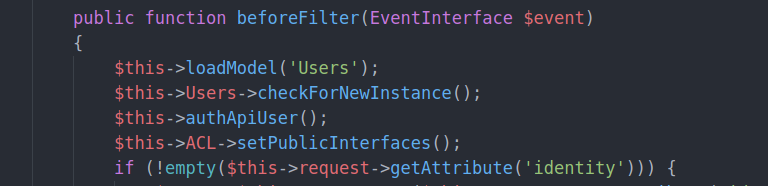
\includegraphics[scale=0.5]{beforefilter.png}
    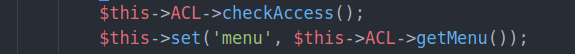
\includegraphics[scale=0.5]{beforefilter2.png}
    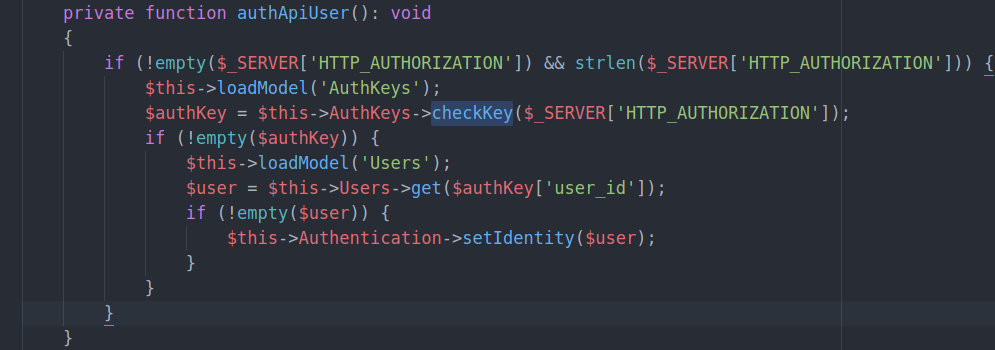
\includegraphics[scale=0.45]{beforefilter3.png}
\end{frame}

\begin{frame}
  \frametitle{Pros of the new system}
  \begin{itemize}
    \item Hashed keys are much more sane for the security posture of the application
    \item Multiple keys are great for auditing (which one of my tools is misbehaving?)
    \item Expirations for ad hoc keys avoids deprecated use-cases having access to the data
  \end{itemize}
\end{frame}

\begin{frame}
  \frametitle{Cons of the new system}
  \begin{itemize}
    \item Definitely slower
    \begin{itemize}
        \item Mostly an issue for stateless, high volumes of requests (MISP)
        \item Using the simple authkeys the lookup is a single indexed select
        \item With that said, the cleartext start/end strings mostly negate this
    \end{itemize}
    \item Users receive their newly generated keys at the end of the creation
    \item There is no way to recover the key if they didn't note it down (but they can always create more)
    \item API keys still need to be stored in the clear for tools connecting to Cerebrate/MISP (even for sync)
  \end{itemize}
\end{frame}


\begin{frame}
  \frametitle{Role based access control}
  \begin{itemize}
    \item The ACL system of MISP and Cerebrate handle all incoming requests
    \item Each user has a role assigned with permission flags
    \item Users 403d whenever they do not have the permission flags required by an action
    \item (Cerebrate only) The menu system is aware of the user's permissions
    \item Restrictive by default
  \end{itemize}
\end{frame}

\begin{frame}
  \frametitle{ACL}
  \begin{center}
    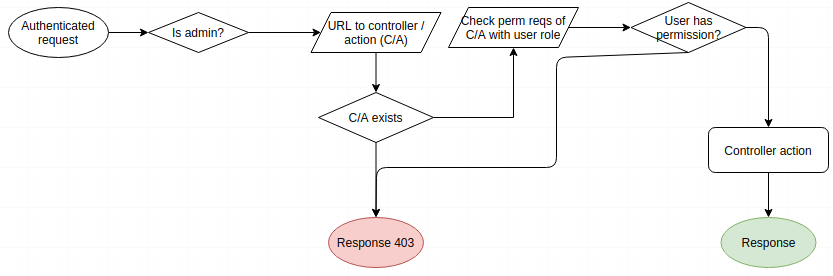
\includegraphics[scale=0.5]{ACL.png}
  \end{center}
\end{frame}

\begin{frame}
  \frametitle{ACL internals}
  \begin{itemize}
    \item All permissions are stored in a large array
    \item The format is Controller-> action -> list of permissions required
    \item Permissions can be combined with logical operators
    \item Wildcards can be used for anything
    \item Empty lists or an endpoint not tied into the ACL will deny all except admins
  \end{itemize}
\end{frame}

\begin{frame}
  \frametitle{ACL list}
  \begin{center}
    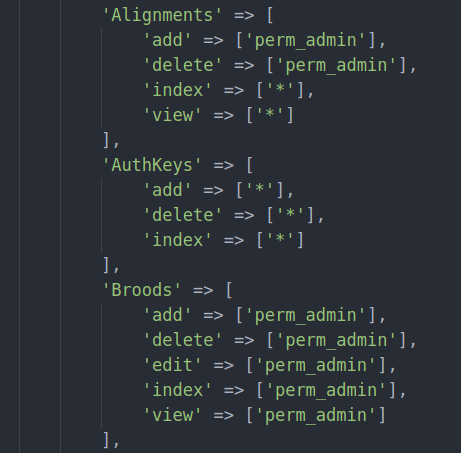
\includegraphics[scale=0.5]{ACLList.png}
  \end{center}
\end{frame}

\begin{frame}
  \frametitle{ACL logic}
  \begin{center}
    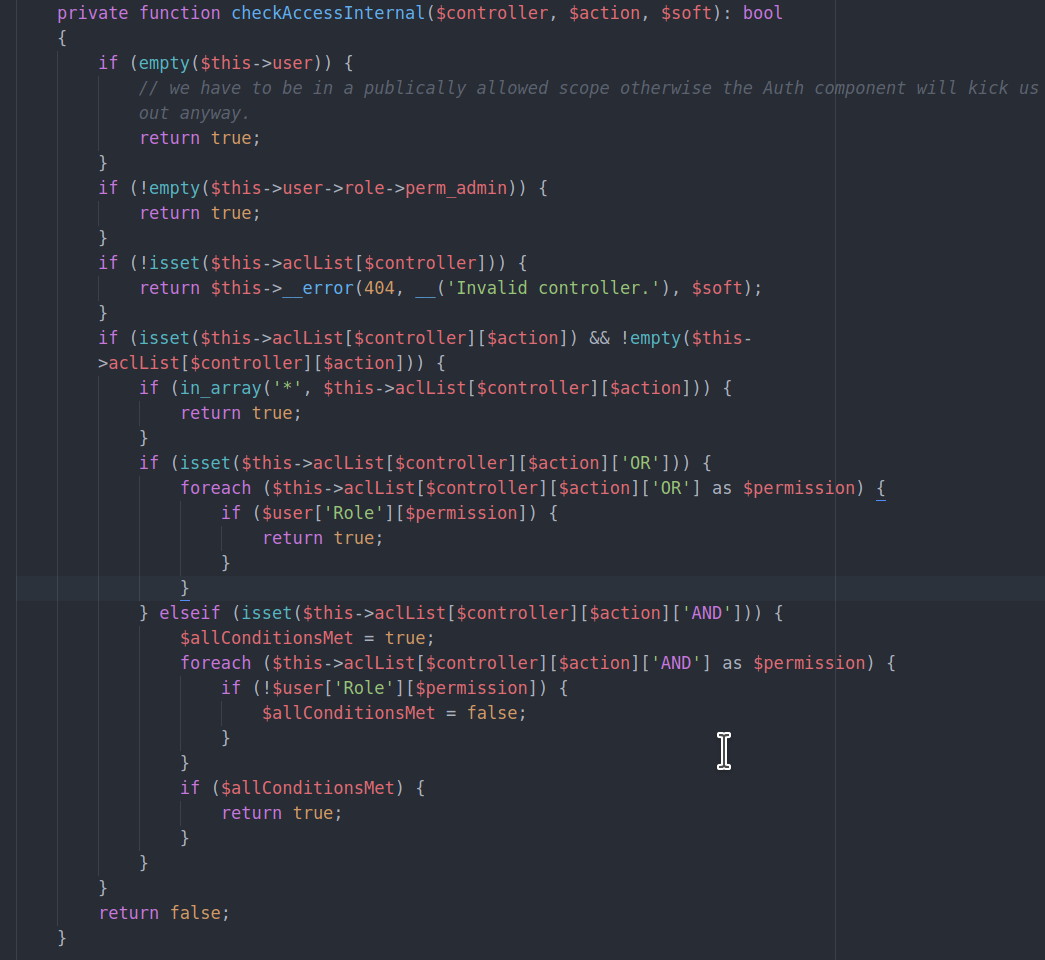
\includegraphics[scale=0.3]{ACLCheck.png}
  \end{center}
\end{frame}

\begin{frame}
  \frametitle{Additional tooling in the ACL package}
  \begin{itemize}
    \item For devs: enumerate endpoints not tied into the ACL (queryACL action)
    \item For integrators: List all urls accessible for a given role
    \item We also use the enumeration as a sanity check in our CI process for MISP (soon Cerebrate)
  \end{itemize}
\end{frame}

\begin{frame}
  \frametitle{queryACL}
  \begin{center}
    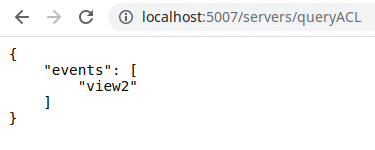
\includegraphics[scale=0.5]{queryACL.png}
    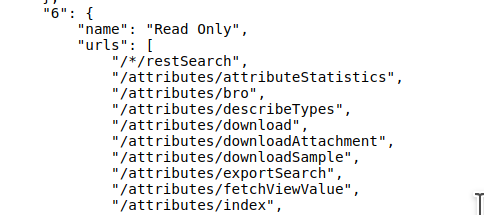
\includegraphics[scale=0.5]{queryACLPrint.png}
  \end{center}
\end{frame}

\begin{frame}
  \frametitle{ACL}
  \begin{center}
    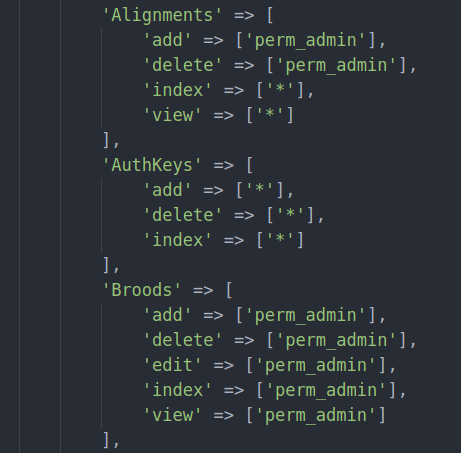
\includegraphics[scale=0.5]{ACLList.png}
  \end{center}
\end{frame}


